\documentclass[UTF8,a4paper,11pt,fontset=fandol]{ctexart}
\usepackage[margin=2.3cm]{geometry}
\usepackage{booktabs,tabularx,amsmath}
\usepackage{graphicx}
\usepackage[section]{placeins}
\usepackage{xurl}
\usepackage[unicode,colorlinks=true,linkcolor=blue,urlcolor=blue,citecolor=blue]{hyperref}
\DeclareRobustCommand{\code}[1]{\nolinkurl{#1}}
\title{oGMemory-m3：面向长视频问答的多模态记忆系统\\架构设计与实验评估}
\author{刘远见}
\date{2026 年 11 月 3 日}
\begin{document}
\maketitle
\begin{abstract}
长视频问答要求将分散的视觉、语音与人物线索转化为可长期保存、按需检索的证据。
本文提出oGMemory-m3，从零设计并实现覆盖媒体感知、情景记忆构建、
来源关联与索引及多轮检索问答的多模态记忆系统。
系统新增记忆图谱存储、算子机制与声明式编排流程，
将各处理模块组织为可配置、可追踪的执行链路。
系统以统一来源组织连接视频片段、结构化事实与回答证据，通过片段与事实的混合召回保留
局部细节，并以来源位置去重和有界增量交付控制重复上下文。
在 M3-Bench 最新已完成实验的八视频、97题配对子集上，使用相同
MiniMax-M3.1-Flash模型、共享感知输入与共同自动评委，
oGMemory获得0.5722的自动评分均值，高于M3-Agent参考适配的0.4381，
并在八个视频中的六个取得更高评分。
我们进一步报告建忆与问答的token开销及阶段耗时，
将质量表现与系统处理成本放在同一评估范围内。
结果展示了来源可追溯、细粒度证据检索和受控上下文交付相结合的应用价值。
\end{abstract}

\section{Introduction}
多模态记忆的目标并非保存尽可能多的原始媒体，而是在有限计算和上下文预算下，
为后续问题保留可定位、可关联的证据。长视频中的回答可能依赖多个时刻的物品变化、
人物偏好、对话内容与视觉状态。直接将全部视频描述和转写拼接给语言模型，
会使无关信息和重复检索结果累积；过早压缩成短摘要，又可能丢失姓名、数量、
动作对象等决定答案的细节。

构建这样的记忆系统需要贯通三个环节。首先，\textbf{多模态感知与记忆表示}需要把
视频帧、语音转写、人物与事件组织到共同的片段和时间坐标中，使不同模态的观察能够联合使用。
其次，\textbf{证据组织与检索}需要兼顾片段背景和局部细节，既能回答某个时刻发生了什么，
也能定位分散在多段对话或画面中的相关事实。最后，\textbf{按需交付与问答}需要将检索结果
转化为语言模型可消费的有界上下文，避免反复发送相同内容，同时允许继续补充证据。

本文从零构建oGMemory-m3多模态记忆系统，设计记忆图谱存储、
算子机制及算子编排流程，接入视频与音频，生成结构化情景记忆，建立来源关系及
多粒度索引，再通过带时间约束的检索与多轮问答使用这些记忆。
本文的工作范围覆盖整条多模态处理链路，而非对一个预先存在的多模态记忆模块进行局部优化。
核心设计包括：
\begin{itemize}
\item \textbf{算子化处理与声明式编排。}新增处理算子的封装、阶段配置与执行机制，
以显式依赖连接感知、记忆、索引和问答，统一记录各阶段产物与执行状态。
\item \textbf{来源贯通的记忆图谱。}新增以节点和关系组织媒体、抽取结果与记忆的存储方式，
保留时间及证据出处，使记忆可检查、检索可回源，并为后续文本记忆迁移提供统一表示。
\item \textbf{兼顾背景与细节的检索。}联合情景片段、转写和原文事实窗口，
结合有来源的人物条件，使局部证据能够在保留片段背景的同时进入问答。
\item \textbf{受控的证据消费。}以已交付的来源位置为粒度增量补充证据，
结合整体输入预算与回答收尾机制，降低多轮检索中的重复输入。
\end{itemize}

我们以相同模型适配的M3-Agent作为对照，在共同感知输入上分别生成记忆、执行问答。
本文只比较两套系统，不展开内部配置消融；以已完成的八视频配对子集报告
逐视频质量、token用量及处理时间，并明确区分已评测版本与仍在复测的新实现。

\section{Related Work}
\subsection{多模态记忆与长视频理解}
长视频记忆的一条路线是在视觉表示层压缩历史信息。MovieChat\cite{moviechat}
以视觉token为记忆载体，借鉴短期与长期记忆机制，将密集视频信息组织为稀疏记忆，
以支持长视频理解。另一条路线把视频转化为可查询的结构化观察。
VideoAgent\cite{videoagent}同时保存时序事件描述和以对象为中心的跟踪状态，
通过片段定位、对象记忆查询等工具，由语言模型交互式求解视频任务。
这些工作分别体现了表示压缩与结构化检索两种设计思路。

M3-Agent\cite{m3agent}进一步面向持续的视听输入，构建以实体为中心的多模态记忆，
同时保存情景事实与高层语义知识，并通过迭代检索进行推理。
其人脸和声音线索参与人物关联，使不同模态中的观察能够围绕人物组织；
配套M3-Bench评估人物理解、跨模态推理等长视频记忆能力。
与仅压缩视觉表示的路线相比，这类系统更关注可持续更新的实体与事实记忆。
本文同样从视频与音频构建记忆，但以源片段、字段位置和时间边界连接结构化证据，
强调检索结果的可回溯性及多轮问答中的细粒度交付。

\subsection{文本记忆与语言智能体}
文本记忆研究为记忆组织和有限上下文管理提供了基础。
Generative Agents\cite{generative}以自然语言保存经历，通过检索和高层反思支持行为规划，
体现了从观察到抽象记忆的组织方式。MemGPT\cite{memgpt}借鉴操作系统分层存储，
在有限上下文和外部记忆之间管理信息流，将上下文管理作为智能体控制的一部分。
二者分别突出记忆内容的组织与工作上下文的调度。

面向长期对话，Mem0\cite{mem0}通过抽取、整合和检索重要信息维护持久记忆，
并提出图式变体表达关系；A-MEM\cite{amem}借鉴卡片笔记法，
为记忆生成结构化属性、建立关联，并随新记忆加入更新既有记忆表示。
这些系统说明，持久记忆不只是扩大提示窗口，还需要选择、关联和维护信息。
但从文本对话迁移到视听输入，还需处理感知误差、时间对齐和人物归属。
本文将来源约束、事实检索与受控上下文连接起来，不把文本相关性直接当作跨模态身份等价。
上述论文用于定位设计，并未全部纳入本次实验对比。

\subsection{与M3-Agent的设计区别}
M3-Agent强调紧凑的情景/语义事实和实体关联；本文在oGMemory中新增的多模态子系统，
将媒体、抽取结果与记忆关联存储，默认QA检索情景节点及其来源事实。
事实窗口保留原文位置，不额外生成高层语义推断；人物条件采用来源中的姓名/角色软排序，
而不是已核实的人脸--声音--姓名链接。

在本文审阅的参考实现中，M3-Agent普通控制路径主要每次取top-2片段，
记录已交付片段并追加新片段；本文按\emph{源位置}去重，允许补充同一片段中尚未看到的事实。
上述控制细节来自本地实现审阅，不是对所有多模态记忆方法的通用假设。
本次对照保留M3-Agent参考控制思路，以共同模型替代其专用记忆和控制权重，
因此是\textbf{同模型参考适配}，不是原论文官方权重或成绩复现。

\section{Method}
\subsection{总体架构与数据流}
系统建立“媒体接入与感知、记忆构建与存储、索引与检索、上下文交付与回答”四层处理链路。
记忆图谱存储、算子机制与声明式编排共同构成从零搭建的系统基础：
图谱层组织原始输入、抽取事实、持久记忆及其关系，算子层实现各类处理，
编排层连接阶段依赖与执行产物。视频/音频处理、情景记忆生成、多模态来源关联、
面向视频的索引检索及问答控制在这一架构中协同工作。
图谱层不将输入限定为视听媒体，为后续文本记忆接入同一记忆表示与关系体系预留路径。
离线构建层把连续媒体转化为持久记忆；在线问答层根据问题和时间范围选择证据，
无需在每次回答时重新处理完整视频。表\ref{tab:architecture}概括模块职责。

\begin{table}[htbp]
\centering\small
\caption{oGMemory-m3的层次与数据流。}
\label{tab:architecture}
\begin{tabularx}{\linewidth}{lXX}
\toprule
层次 & 主要处理 & 输出与接口\\
\midrule
媒体感知 & 视频切片、帧与音频提取、转写、人物线索 & 带片段及时间来源的媒体与观察\\
记忆图谱 & 情景抽取、节点与关系存储、视频级整合 & 原始输入、事实、记忆及来源和支持关系\\
索引检索 & 片段/事实向量、转写召回、人物软排序 & 经账号、视频、时间与哈希校验的证据\\
检索问答 & Search/Answer循环、增量交付、预算控制 & 可回溯证据的回答及运行记录\\
\bottomrule
\end{tabularx}
\end{table}

\subsection{算子机制与声明式编排}
新增算子机制将媒体处理、特征抽取和记忆生成等操作封装为可调用单元，
编排层通过注册的阶段处理函数将这些操作与存储、索引和问答步骤连接起来。
阶段描述声明标识、类型、启用状态、参数与依赖；共享运行上下文传递媒体产物路径、
账号和视频范围、图存储及索引服务。算子负责具体处理，编排层负责阶段衔接与执行记录，
二者共同构成本文新增的处理框架。

流程采用声明式配置，而非在单一脚本中固定全部调用。
例如，情景记忆生成依赖帧提取、音频提取和转写，记忆节点创建与索引构建依赖情景抽取结果。
执行器检查阶段类型及依赖是否有效，在执行阶段前检查其前置状态，
并统一记录输出、计数、错误和警告；可选阶段通过配置启停。
对于具有完成性探测的阶段，可检查已有产物后跳过重复执行。
这使处理配置与算子实现分离，便于替换组件、定位失败及恢复执行；
它是系统架构能力，本文不将其单独归因为问答得分提升。

\subsection{有界并行执行}
针对媒体处理和远程调用的等待开销，系统在保持阶段依赖顺序的前提下，
将阶段内部相互独立的工作交给有界线程池：
帧和音频提取、人脸检测及远端情景记忆生成按视频片段分派，
限制工作线程和排队任务数量；各片段独立记录成功、失败与重试，
结果由主线程汇总并按输入顺序整理。问答则以问题为单位并发，
每个工作线程使用独立的适配器和检索状态，完成后按问题标识及时写出结果，
避免等待最慢的问题，也避免不同问题的上下文和预算相互干扰。

共享的图谱及向量连接通过连接池管理，嵌入请求以信号量限制并发；
这些限制作用于单个进程，不能视为跨进程的全局配额。
本地GPU上的转写、说话人分离及声纹提取仍串行执行，以避免重复加载模型占用显存。
一次并行复测配置采用单视频、片段抽取4、人脸检测2、情景记忆8、问答4及嵌入4的并发上限；
具体配置可调整，并非所有视频同时处理。并发主要用于减少等待时间，
不天然降低token消耗或保证输出质量一致，实际收益还受服务限流及共享资源瓶颈影响。
该机制属于后续集成，不改变本文已有实验结果的运行口径。

\subsection{媒体感知与结构化情景抽取}
视频按30秒切片，每段创建视频源节点，并关联抽取的图像帧及16 kHz单声道音频。
视觉处理提取帧及人脸线索；音频处理使用Whisper转写、pyannote说话人分离及ECAPA声纹特征。
图像、可用音频和转写进入情景记忆生成算子，形成包含description、characters、events和
entities的片段级结构化输出，分别记录场景描述、人物、事件及实体。
这一表示将视觉观察与对话内容置于同一片段背景下，为后续文本化检索提供统一入口。
每个30秒片段按1 fps收集至多30帧，再从整个采集序列均匀选取至多16张基础模型帧；
标准片段的模型输入时间范围约为0--28秒，而非仅覆盖前16秒。
这一规则改善时间覆盖，但仍可能遗漏短暂动作或细小视觉线索。

片段处理保留独立状态和失败清单。无效结构化输出可有限重试，
仍失败的片段被显式记录；继续处理其他片段后按覆盖门槛判断整体是否合格，
避免单片段故障直接中断全部视频，也不把缺失片段伪装成完整记忆。

\subsection{记忆图谱存储、人物线索与时间约束}
本文新增记忆图谱存储方式，以节点表达不同层次的信息，以关系表达来源、支持和演化。
在多模态流程中，原始媒体作为Raw节点，结构化抽取作为Extracted节点，
持久记忆作为Memory节点，三者通过来源及支持关系连接。
图谱提供结构化事实及证据链的组织方式，向量与词法索引提供按问题检索的入口，
两者分别承担关联存储与相关性召回。问答默认检索情景抽取节点，
并可由节点及字段位置返回原片段。视频级记忆通过描述拼接和集合去重整合，
维护支持与演化关系；它不额外生成高层语义推断。
人脸和声音聚类保留人物关联线索，但这不等于已核实的跨模态姓名绑定，
也不意味着默认QA直接遍历所有身份关系。

所有检索受账号、视频和可用时间限制。本文实验采用\code{current_clip}协议，
允许使用问题所在片段末尾之前的证据；事实可用时间保守地取其来源片段末尾，
不读取未来片段建立姓名映射。由于该边界可能晚于问题时刻，
本文不将这一设置称为严格因果在线问答。

\subsection{来源事实索引与混合召回}
我们将源记忆拆成三类窗口：description 的局部原文、相邻三条ASR转写，以及完整的
事件、人物或实体项。每个窗口记录源节点、字段位置或字符范围、内容哈希及可用时间。
相同文本在不同时间出现仍是不同观察；窗口数不能直接当作事件发生次数。

每个视频的来源窗口由 BGE-M3 编码为1024维向量，并形成独立的事实索引。
检索层并行使用片段向量、转写和事实窗口召回；事实命中按最大分数聚合到源节点，
再与片段及转写候选排序等权融合：
\[
 \operatorname{RRF}(d)=\sum_{r\in\mathcal{R}}\frac{1}{k+\operatorname{rank}_{r}(d)}.
\]
其中 $\mathcal{R}$ 表示参与融合的排序，$k$ 为平滑常数。
候选进入上下文前需再次验证范围与源内容哈希，避免旁路索引绕过权限或引用过期内容。
该索引是面向小规模固定数据的密集检索原型，而非生产级ANN或动态语义图。

\subsection{显式人物条件软排序}
在已通过范围过滤的候选内，查询若完整匹配来源中的 name 或 role，
则给予有限的排序奖励，并提高对应人物描述的准入优先级。
我们不硬性排除无匹配候选，避免将“没有写姓名”误当成“不属于此人”。
局部 \code{SPEAKER_00} 等标签不作为跨片段身份，角色相同也不自动合并人物。
这是一种来源声明驱动的检索条件，而不是身份识别算法。

\subsection{严格增量证据交付与回答收尾}
每题维护已实际发送的来源位置集合 $D_t$。第 $t$ 轮检索的候选事实为 $C_t$，
只从 $C_t\setminus D_t$ 中选入新证据；过去的工具消息保持不变。
这种去重既减少整片段重传，也允许补充同源片段的不同事实。
停搜依据实际新增可见事实，而非仅检查是否出现新节点。

本次评测配置将每轮新增额度设为3500，按照实际模型投影的token估计计数，
不把未发送的审计字段计入额度基数。全部历史还受整体有效输入预算约束：
\[
 B_{\mathrm{input}}=32768-8192-2048=22528,
\]
分别为操作窗口、输出预留与安全余量。单次新增节点上限不等于整个历史的节点上限；
必要时可重建上下文并重置交付集合。
收尾时仅提供 Answer 工具并请求必选；普通文本仍由既有兼容路径接收，
因此该设置不是严格的原生工具输出保证。

\section{Evaluation}
\subsection{数据、模型与评测范围}
实验来自M3-Bench\cite{m3agent}的robot子集：原五个开发视频之外，
从剩余视频中以seed=42随机抽取五个扩展视频，预先固定十视频、128题。
主分析沿用执行顺序中的前八视频，共97题，包含五个扩展视频和三个原开发视频。
两方法在这些视频上完成记忆构建及整套QA执行；\code{kitchen_01}的两道原始超时题
仍计零，不以之后重跑的答案替换，也不删除该视频。
\code{study_18}的M3路径出现11道连接失败，\code{kitchen_20}因上游embedding失败
未完成两方法问答，故不进入主配对子集。完整128题仍保留失败计零的记录：
oGMemory和M3均分分别为0.4805和0.3320，有效回答为109/128和100/128；
该总体差异受到服务故障影响，不作为主要算法质量结论。

两方法共享本轮新生成的基础帧、完整音频及转写，分别独立生成记忆和执行QA。
记忆生成、QA与评委均配置MiniMax-M3.1-Flash，
\code{thinking=adaptive}、\code{reasoning_effort=medium}；QA输出上限8192、
评委2048，最多6轮及180秒软预算。oGMemory使用来源事实索引与严格增量3500配置；
M3-Agent保留参考Action文本控制协议，以共同模型替代专用训练权重。
双方基础模型帧最多16张，M3可额外输入至多8张人脸裁剪。
本轮逐视频执行，两方法记忆生成均为4并发，QA均串行。

本节对应已完成实验冻结版本\code{8d61b772}，使用全片段采样。
后续人物绑定和并发版本的复测尚未形成完整对照，不与本节混合。
所有分数统一取最终十视频共同评委批次：256个方法--问题对按seed=1102交错，
评委不接收方法名，无评委错误。每题$s_i\in\{0,0.5,1\}$，
主指标为$S=\frac{1}{97}\sum_{i=1}^{97}s_i$，另列全分题比例和有效回答数。
这是\textbf{自动评分，而非人工准确率}；不混用早期八视频临时评分。

\subsection{同模型质量对比}
表\ref{tab:videos}与图\ref{fig:scores}展示全部八个视频。
oGMemory题目加权均分为0.5722，M3-Agent为0.4381，分差为0.1340；
oGMemory在六个视频上更高，在\code{gym_03}上持平，
在\code{kitchen_23}上较低。因而总分优势不是逐视频全面占优。
有效回答分别为95/97和97/97；覆盖率、自动评分与事实正确性应分开解释。

逐视频看，\code{bedroom_04}和\code{study_23}的分差最大，分别为36.4和35.7个百分点；
两者合计贡献9个评分点，占全部97题累计分差13点的约69.2\%。
去除这两个视频后，其余72题上的平均分差为5.6个百分点。
这说明总体优势受到少数视频的较大分差影响，不能将整体均值视为每个视频上的典型提升。
同时，\code{kitchen_23}上oGMemory落后8.3个百分点，\code{gym_03}上两者持平，
表明不同视频上的相对表现存在差异。

从评分构成看，oGMemory和M3-Agent的全分题比例分别为51.55\%和37.11\%，
前者高14.44个百分点；但该指标与包含半分题的平均分衡量的内容不同。
每个视频仅有11--14题，少量题目的评分变化即可明显影响逐视频比例；
上述结果因此适合描述本次样本的表现，不足以推断差异的统计显著性或具体成因。

% Generated by scripts/build_m3_paper_comparison.py; final common judge only.
\begin{table}[htbp]\centering\small
\caption{已完成配对子集的逐视频自动评分。保留全部97题；失败计零。}
\label{tab:videos}\begin{tabular}{lrrrr}\toprule
视频 & 题数 & oGMemory & M3-Agent & 分差\\\midrule
\code{study_09} & 12 & 0.5833 & 0.5000 & +0.0833\\
\code{kitchen_01} & 13 & 0.3846 & 0.1923 & +0.1923\\
\code{bedroom_05} & 12 & 0.4167 & 0.3750 & +0.0417\\
\code{study_23} & 14 & 0.6786 & 0.3214 & +0.3571\\
\code{kitchen_23} & 12 & 0.5417 & 0.6250 & -0.0833\\
\code{study_05} & 12 & 0.4583 & 0.3750 & +0.0833\\
\code{gym_03} & 11 & 0.7273 & 0.7273 & +0.0000\\
\code{bedroom_04} & 11 & 0.8182 & 0.4545 & +0.3636\\
\midrule
题目加权合计 & 97 & 0.5722 & 0.4381 & +0.1340\\
\bottomrule\end{tabular}\end{table}
\begin{figure}[htbp]\centering
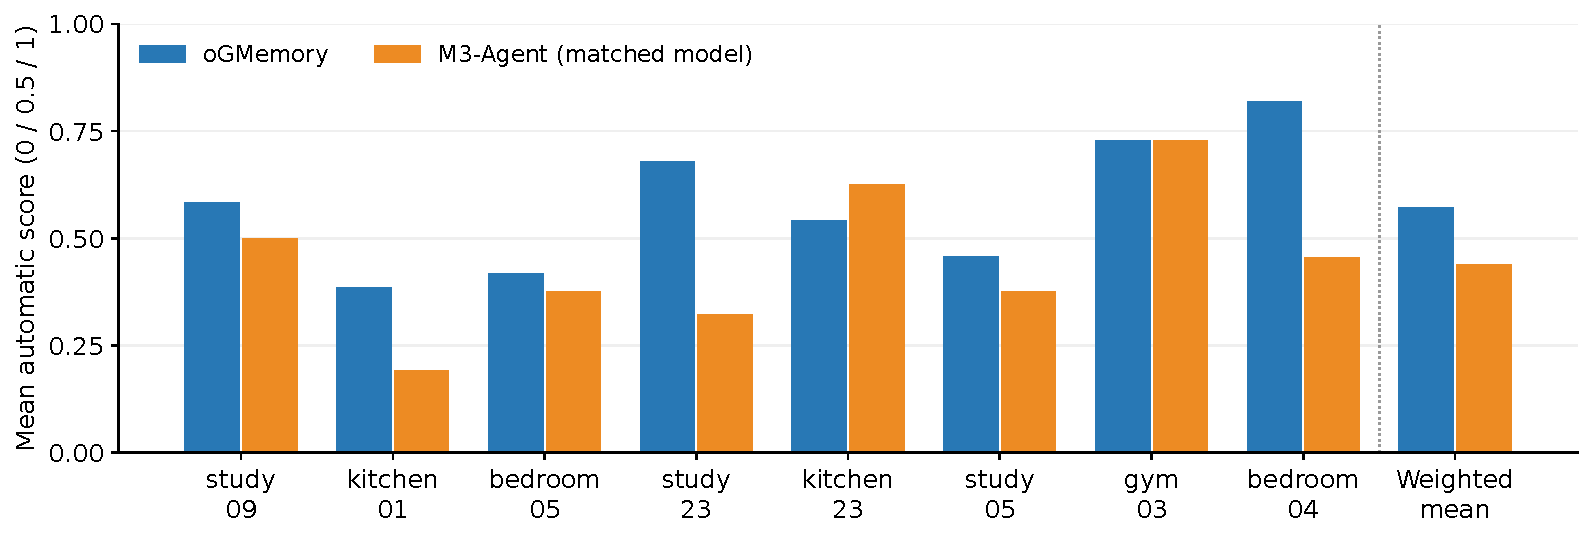
\includegraphics[width=\linewidth]{figures/paired8_final_scores.pdf}
\caption{两方法逐视频表现及题目加权均值。纵轴为自动评分而非人工准确率；不拼接早期临时评分或重跑答案。}\label{fig:scores}\end{figure}
\begin{table}[htbp]\centering\small
\caption{同一八视频子集的质量与资源开销。M为百万token，时间单位为分钟。}
\label{tab:resources}\begin{tabular}{lrr}\toprule
指标 & oGMemory & M3-Agent\\\midrule
有效回答 & 95/97 & 97/97\\
全分题比例（\%） & 51.55 & 37.11\\
QA输入（M） & 4.039 & 0.734\\
其中未缓存输入（M） & 2.129 & 0.263\\
QA输出，含推理（M） & 0.112 & 0.045\\
已记录建忆+QA总token（M） & 7.446 & 4.399$^{*}$\\
共享感知与启动 & 49.02 & 49.02\\
记忆、图谱及索引 & 573.46 & 249.64\\
QA耗时 & 65.91 & 31.02\\
各自计入感知后的总时间 & 688.39 & 329.68\\
\bottomrule\end{tabular}
\par\smallskip\footnotesize $^{*}$M3建忆有1次失败请求未返回usage，该总量仅表示已记录用量，不把未知值当作零；两方法QA用量完整。
\end{table}
\begin{figure}[htbp]\centering
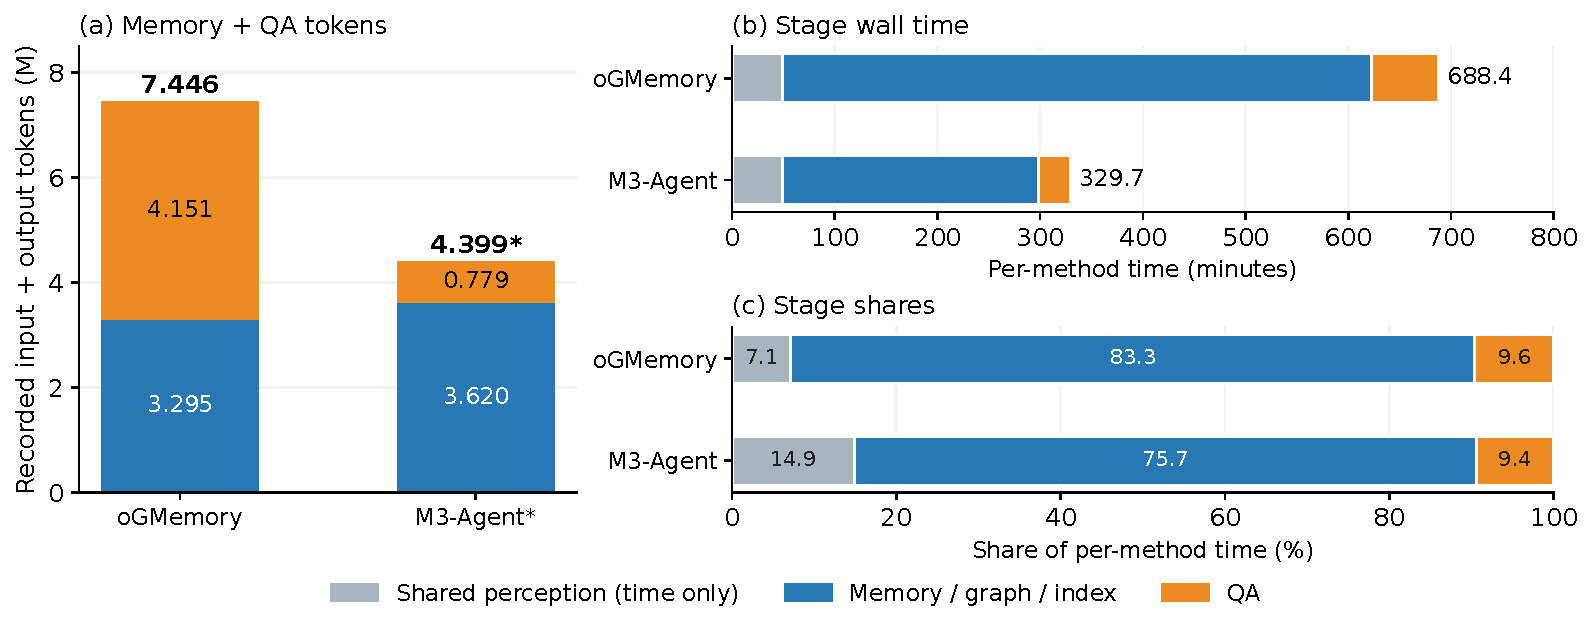
\includegraphics[width=\linewidth]{figures/paired8_final_resources.pdf}
\caption{资源开销及阶段分布。左图为建忆与QA已记录的输入、输出总token，不含embedding和评委；星号表示M3有未知建忆用量。右图将同一次共享感知分别计入两条方法路径；占比由累计耗时计算，不能将两方法总时间相加当作实验墙钟时间。}\label{fig:resources}\end{figure}


\subsection{Token开销与阶段耗时}
表\ref{tab:resources}及图\ref{fig:resources}使用同一97题集合。
QA用量覆盖所有调用，输入包含缓存部分，输出包含推理token，不重复计数；
建忆与QA合计不包含embedding及最终评委。M3建忆有一次失败调用未返回usage，
图中星号总量仅为已记录值，未知部分未估算为零。

oGMemory的QA输入为4.039M，M3为0.734M，前者约为后者的5.50倍；
未缓存输入分别为2.129M和0.263M。oGMemory保留丰富的来源证据，
但当前结果仍表现为\textbf{更高自动评分与更高问答输入开销的折中}，
不能据此宣称比M3更省token。输入比例也不等于实际账单费用比例。

两方法分别计入同一份共享感知后，处理时间为688.39与329.68分钟。
耗时统计采用阶段墙钟边界，包含初始化、等待与重试，不含最终评委及阶段间调度空隙。
共享感知实际只执行一次，分摊到各方法用于独立路径比较，不能重复相加为实验总时长。
记忆、图谱与索引占两方法各自耗时的83.3\%和75.7\%，均为主要开销。
oGMemory该阶段中，旧实现重复处理账号累计人脸耗时309.29分钟，
约占其总时间的44.9\%；因此这些时间反映所测实现，而非单个独立视频的固有建忆成本。
M3建忆封装了身份组织、生成与embedding，不能可靠地进一步拆成纯模型计算时间。

\subsection{解释边界}
主子集不是独立留出测试，也不是对所有服务故障免疫的完整十视频对照。
每方法仅一条完整配对轨迹，未据此宣称统计显著或稳定泛化增益。
共同模型与共享感知改善了可比性，但两者的身份裁剪、记忆组织及控制协议仍不同：
M3末轮允许合理猜测，oGMemory强调证据不足时说明。
此外，\code{current_clip}允许使用问题所在片段末尾的证据，不等于严格因果在线问答。
分差不能单独归因于存储结构、某个算子或人物身份推理。

\section{Conclusion and Discussion}
本文从零构建oGMemory-m3，以新增记忆图谱存储、算子机制与声明式编排，
贯通媒体感知、情景抽取、来源关联、混合检索及多轮问答。
在最新已完成实验的八视频配对子集上，oGMemory相对同模型M3-Agent参考适配
取得更高的自动评分，并以来源位置保存可检查的证据；与此同时，
问答token与处理时间仍更高。质量、输入开销和阶段成本应联合报告，
不能只用单一平均分评价系统。

全片段均匀采样改善了时间覆盖，但稀疏帧、ASR误差、人物归属和事件计数
仍可能限制记忆质量，检索不能补回未被感知的事实。
阶段耗时揭示了身份处理与建忆环节的优化空间；后续人物关联和并发实现
需要在同一完整题集上重新评测，不能将其预期收益归入本文已有结果。
进一步应扩展独立视频样本，引入人工抽查或独立评委，并通过受控消融
区分各算子的贡献。

记忆图谱也是面向文本记忆的共享存储设计。未来可将对话或文档作为源节点，
将文本抽取事实和已有记忆映射到图谱，补建来源与支持关系，逐步迁移文本记忆。
该迁移仍需验证历史来源、时间映射和检索兼容性，本次评测不声称已验证文本迁移收益。

\begin{thebibliography}{9}
\bibitem{moviechat} Enxin Song, Wenhao Chai, Guanhong Wang, et al.
MovieChat: From Dense Token to Sparse Memory for Long Video Understanding.
\textit{CVPR}, 2024. arXiv:2307.16449.
\bibitem{videoagent} Yue Fan, Xiaojian Ma, Rujie Wu, et al.
VideoAgent: A Memory-augmented Multimodal Agent for Video Understanding.
\textit{ECCV}, 2024. arXiv:2403.11481.
\bibitem{m3agent} Lin Long, Yichen He, Wentao Ye, et al.
Seeing, Listening, Remembering, and Reasoning: A Multimodal Agent with Long-Term Memory.
arXiv:2508.09736, 2025.
\bibitem{generative} Joon Sung Park, Joseph C. O'Brien, Carrie J. Cai, et al.
Generative Agents: Interactive Simulacra of Human Behavior.
arXiv:2304.03442, 2023.
\bibitem{memgpt} Charles Packer, Sarah Wooders, Kevin Lin, et al.
MemGPT: Towards LLMs as Operating Systems.
arXiv:2310.08560, 2023.
\bibitem{mem0} Prateek Chhikara, Dev Khant, Saket Aryan, Taranjeet Singh, Deshraj Yadav.
Mem0: Building Production-Ready AI Agents with Scalable Long-Term Memory.
arXiv:2504.19413, 2025.
\bibitem{amem} Wujiang Xu, Zujie Liang, Kai Mei, Hang Gao, Juntao Tan, Yongfeng Zhang.
A-MEM: Agentic Memory for LLM Agents.
\textit{NeurIPS}, 2025. arXiv:2502.12110.
\end{thebibliography}
\end{document}
